\section{Evaluation} \label{sec:eval}

We address two problems in our experiments :
\begin{itemize}
	\item Mapping a SQL workload to a benchmark class.
	\item Estimating the performance of the DBMS using the features and the class
	model.
\end{itemize}

We note that we leave the problem of using the performance estimator to find
an optimal DBMS configuration for a given workload for future work. The
estimator allows us to obtain inexpensive estimates without actually running
the workload on the DBMS under a specific configuration.


\begin{table*}
\centering
  \begin{adjustbox}{max width=\textwidth}
  \begin{tabular}{l|lll} 
	\toprule
   		Feature name &  Feature meaning & Default value & Mutated value set \\
    \midrule
    	shared\_buffers & Number of shared memory buffers used by the database
    	server & 128 MB &  [ 4 MB, 32 MB, 128 MB, 512 MB ] \\
    	bgwrite\_delay &  Delay between rounds for the
    	background writer & 100 ms &  [ 100 ms, 1000 ms, 10000 ms ] \\
    	wal\_level & Type of logging & minimal &  [ minimal, archive, hot\_standby,
    	logical ] \\
    	fsync & Forced synchronization to disk & on &  [ on, off ] \\
    	synchronous\_commit & Whether transaction commit will wait for WAL records to be flushed & on &  [ on, off, local,
    	remote\_write ] \\
    	wal\_buffers & Number of disk-page buffers in shared memory for WAL & 
    	-1 &  [ -1, 4 MB, 32 MB, 128 MB ] \\
    	wal\_writer\_delay & Specifies the delay between rounds for the
    	WAL writer & 200 ms &  [ 100 ms, 200 ms, 1000 ms, 10000 ms] \\
    	commit\_delay & Time delay between writing a commit record to the WAL
    	buffer & 0 $\mu$s &  [ 0 $\mu$s, 1000 $\mu$s, 1000 $\mu$s, 10000 $\mu$s] \\
    	track\_activities & Collect query/index statistics  & on &  [ on, off ]	\\
    	log\_planner\_stats & Log planner statistics  & off &  [ on, off ] \\
    	debug\_print\_plan & Print plans in log  & off &  [ on, off ] \\
    	autovacuum & Enable autovacuum subprocess  & on &  [ on, off ] \\    	    	
   \bottomrule
   \end{tabular}
   \end{adjustbox}   
\caption{Configuration attributes that we mutate in each DBMS run.}
\label{tab:mutate}
\end{table*}

We first describe the experimental setup and information about the dataset
in \cref{sec:setup}. Then, we present the results for the
workload mapping/classification problem in \cref{sec:classfication} and for the
performance estimation problem in \cref{sec:estimation}. Finally, we discuss
the conclusions and future work in \cref{sec:conclusion}.

\begin{figure*}
    \centering
    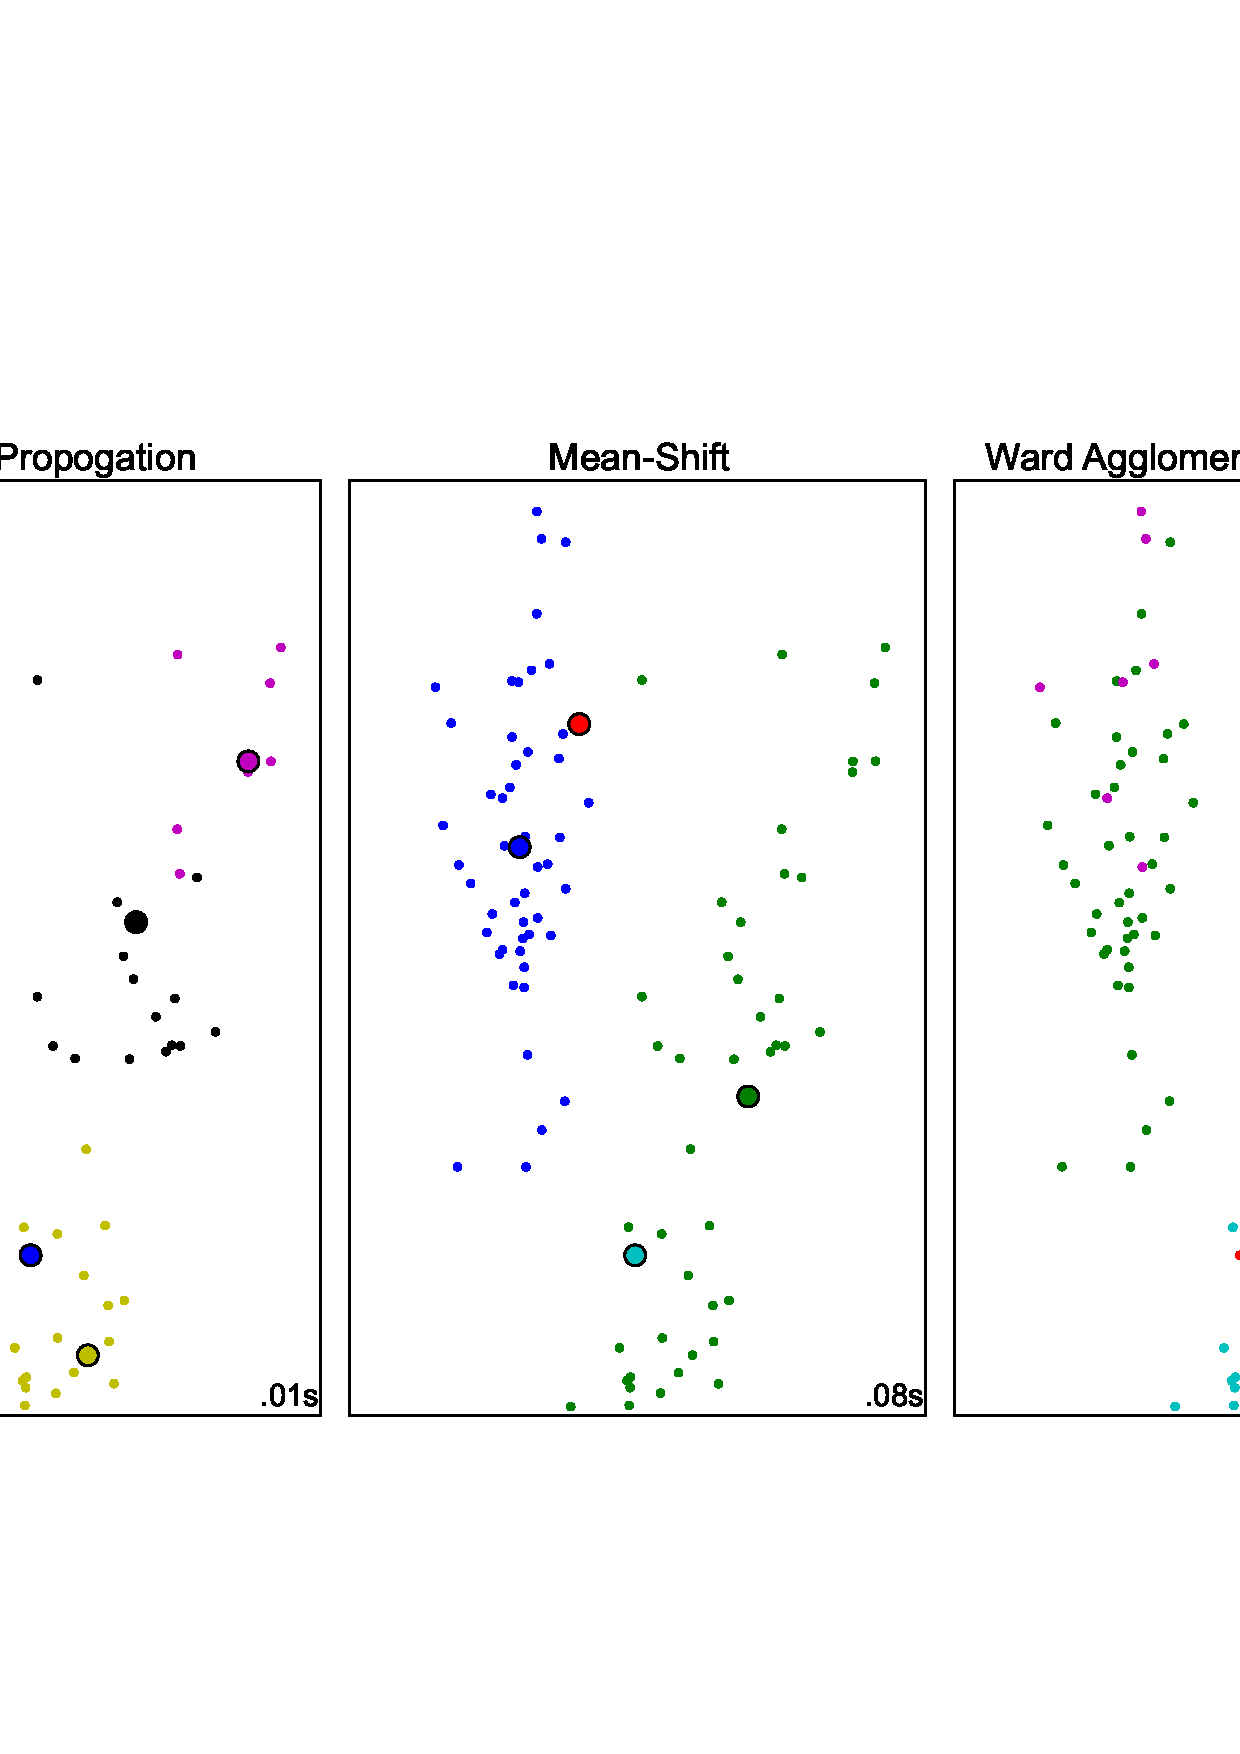
\includegraphics[width=\textwidth]{figure/clustering.pdf}
    \caption{Clusters found by the clustering algorithms.}
    \label{fig:clusters}
\end{figure*}

\begin{figure*}
    \centering
    \begin{adjustbox}{max width=\textwidth}    
    \begin{tabular}{llllll}
      \toprule
      Algorithm                     & Homogeneity & Completeness & V-Measure &
      \# of clusters & Silhouette Coefficient \\
      \midrule
      K-Means                       & 0.607       & 0.592        & 0.600   & 10
      & 0.106  \\
      Affinity-Propagation          & 0.654       & 0.317        & 0.427   & 88 
      & 0.082  \\
      Mean-Shift                    & 0.012       & 0.368        & 0.024   & 2
      & 0.517 \\
      Ward Agglomerative Clustering & 0.589       & 0.635        & 0.611   & 10 
      & 0.097 \\
      \bottomrule
    \end{tabular}
    \end{adjustbox}
    \caption{Performance metrics of clustering algorithms.}
    \label{fig:clustering-metrics}
\end{figure*}

\subsection{Experimental Setup}
\label{sec:setup}

All our experiments are performed on the machine described in \cref{tab:setup}.
We deploy Linux kernel 3.2.0 on the machine and disable logical processor
support (“Hyper-Threading”).
We use the Scikit \citep{scikit-learn} framework in Python 3 for
evaluating different machine learning algorithms.
Our auto-tuning framework currently only supports Postgres 9.5. We plan to
extend it to support other database management systems like MySQL in future
work.

\begin{table}
\centering
\small{
  \centering
  \begin{tabular}{l|l} 
	\toprule
   		Attribute &  Value  \\    
    \midrule
		CPU   &   8 cores (Intel i7-3770 @ 3.7 GHz)  \\
		DRAM   &  16 GiB  \\
		L2 cache  &  256 KiB  \\
		L3 cache  &  8 MiB  \\		
   \bottomrule
   \end{tabular}
 }
\caption{Experimental setup.}
\label{tab:setup}
\end{table}

The dataset consists of 10 benchmark classes. These include all the benchmarks
described in \cref{tab:benchmarks}. We consider 4 variants of the YCSB key-value
store benchmark. These variants map to different read-write mixtures and are
listed below :

\begin{itemize}
  \item {Read-only : 100\% reads 0\% writes } 
  \item {Read-heavy : 80\% reads 20\% writes } 
  \item {Balanced : 50\% reads 50\% writes } 
  \item {Write-heavy : 20\% reads 80\% writes } 
\end{itemize}

We added these variants to stress-test the classifiers and estimators as these
variants can overlap with other benchmark classes along some dimensions in
high-dimensional space. 

For each DBMS run, we first generate a configuration by picking
values for 12 key configuration parameters listed in \cref{tab:mutate}.
We then select a random benchmark and alter the transaction mix of the
benchmark i.e. the proportion of different types of transactions in 
the specific benchmark. After running the benchmark for atleast more than
1 minute, we halt the system.  We then collect the dynamic features from the
DBMS and the benchmarking framework. We also collect the static features
from the specific DBMS configuration. These features and metrics constitute
one sample in the dataset.
Each sample consists of 272 features and our dataset consists of 1000
such samples.

